\documentclass{article}
\usepackage{graphicx} % Required for inserting images
\usepackage{minted}
\newcommand{\pder}[2][]{\frac{\partial#1}{\partial#2}}
\newcommand{\spder}[2][]{\frac{\partial^2#1}{\partial#2^2}}
\newcommand{\tpder}[2][]{\frac{\partial^3#1}{\partial#2^3}}
\newcommand{\fpder}[2][]{\frac{\partial^4#1}{\partial#2^4}}

\title{Numerical Analysis of the Laplace Equation}
\author{Alex Zhou}
\date{May 2019}

\begin{document}

\maketitle

\section{Introduction}

In this article, we shall consider solving the Laplace equation in two dimensions to compute properties of a simple capacitor. The capacitor consists of two parallel rectangular plates of size \(\ell_x \times \ell_z\), separated by distance \(d\). The thickness of the plates is negligible. Let the electric potential at position \((x,y,z)\) be \(\varphi(x,y,z)\). The centres of the plates are at \((x,y,z) = (0,\pm d/2,0)\). On the top plate, \(\varphi = +V/2\) and on the bottom plate, \(\varphi = -V/2\). We shall find a function \(\phi(x,y)\) which solves 
\[ \spder[\phi]{x} + \spder[\phi]{y} = 0, \]
subject to the boundary condition
\[ \phi = (\pm V/2) \mbox{ on the plates: } y = (\pm d/2) \mbox{ and } |x| \leq (\ell_x/2), \]
and boundary at infinite condition
\[ \phi \to 0 \mbox{ as either } |x| \to \infty \mbox{ or } |y| \to \infty. \]
Assume that \(\ell_z \gg \ell_x\). Then the solution \(\phi(x,y)\) is an accurate approximation of \(\varphi(x,y,0)\), which is the potential in the plane \(z = 0\). The electric field in this plane is given by
\[ \mathbf{E} = -\nabla \phi = \left(-\pder[\phi]{x}, -\pder[\phi]{y} \right). \]
For any domain \(\Omega \subset \mathbf{R}^2\) that contains exactly one of the plates, the integral
\[ q = \epsilon_0\int_{\partial \Omega}(\mathbf{E}\cdot\mathbf{n})\,dS. \]
If \(\Omega\) includes all of the top plate, then this gives the charge of the plate per unit length along the \(z\) direction. The capacitance is therefore \(C = q\ell_z/V\). Here, \(\partial \Omega\) is the boundary of \(\Omega\) and \(\mathbf{n}\) is the outward pointing normal to this boundary. The constant \(\epsilon_0\) is the permittivity of free space.

Define the dimensionless units,
\[ X = \frac{2x}{d}, \quad Y = \frac{2y}{d}, \quad L = \frac{\ell_x}{d}, \quad \Phi = \frac{\phi}{V}, \quad Q = \frac{q}{\epsilon_0V}, \]
where \(q\) is computed for the top plate. This simplifies the problem to
\[ \spder[\Phi]{X} + \spder[\Phi]{Y} = 0, \]
with \(\Phi = \pm\frac{1}{2}\) on the plates \(Y = \pm 1\) with \(|X| \leq L\) and \(\Phi \to 0\) far from the plates. 

For large \(L\), the expected physical behaviour in the gap between the plates is that \(\nabla \Phi\) is almost aligned with the \(Y\) direction and depends weakly on \(X\) and \(Y\).

\section{Numerical Method}

We solve the Laplace equation on a rectangular domain \(\mathcal{D} = [-D_X, D_X] \times [-D_Y, D_Y]\), where \(D_X, D_Y\) are appropriately chosen parameters. Set \(\Phi = 0\) on the boundary of this domain (corresponding to putting the capacitor inside a conducting box at potential \(\phi = 0\)). The solution of the original problem is recovered by sending \(D_X,D_Y \to \infty\). We have the symmetries
\[ \Phi(-X,Y) = \Phi(X,Y) \quad \Phi(X,-Y) = -\Phi(X,Y), \] 
so it suffices to compute \(\Phi\) in the positive quadrant of \(\mathcal{D}\).

Define a grid of points \((X_m, Y_n) = (mh, nh)\) for \(m,n\in\mathbf{Z}\) and some grid spacing \(h > 0\). Choose \(\mathcal{D}\) such that \(N_x = D_x/h\), \(N_y = D_y/h\) and \(1/h\) are integers. We now compute a numerical approximation \(\Phi_{m,n}\) to \(\Phi(X_m, Y_n)\) defined by
\[ \Phi_{i-1,j} + \Phi_{i+1,j} + \Phi_{i,j-1} + \Phi_{i,j+1} - 4\Phi_{i,j} = 0. \]

The Taylor expansion for \(\Phi(X_i + h, Y_j)\) is
\[ \Phi(X_i + h, Y_j) = \Phi_{i,j} + h\pder[\Phi]{X} + \frac{h^2}{2!}\spder[\Phi]{X} + \frac{h^3}{3!}\tpder[\Phi]{X} + \frac{h^4}{4!}\fpder[\Phi]{X} + O(h^5), \]
and the Taylor expansion for \(\Phi(X_i - h, Y_j)\) is
\[ \Phi(X_i - h, Y_j) = \Phi_{i,j} - h\pder[\Phi]{X} + \frac{h^2}{2!}\spder[\Phi]{X} - \frac{h^3}{3!}\tpder[\Phi]{X} + \frac{h^4}{4!}\fpder[\Phi]{X} + O(h^5), \]
which sum to
\[ \Phi(X_i + h, Y_j) + \Phi(X_i - h, Y_j) = 2\Phi_{i,j} + 2\frac{h^2}{2!}\spder[\Phi]{X} + 2\frac{h^4}{4!}\fpder[\Phi]{X} + O(h^6). \]
Using \(\Phi_{i+1,j} = \Phi(X_i + h, Y_j)\) and \(\Phi_{i-1,j} = \Phi(X_i - h, Y_j)\),
\[ \Phi_{i+1,j} + \Phi_{i-1,j} - 2\Phi_{i,j} = h^2\spder[\Phi]{X} + \frac{h^4}{12}\fpder[\Phi]{X} + O(h^6). \]
Similarly, considering the Taylor expansion in the \(Y\) direction,
\[ \Phi_{i,j+1} + \Phi_{i,j-1} - 2\Phi_{i,j} = h^2\spder[\Phi]{Y} + \frac{h^4}{12}\fpder[\Phi]{Y} + O(h^6). \]
Altogether, by dividing the central difference approximation by \(h^2\),
\[ \frac{\Phi_{i+1,j} + \Phi_{i-1,j} - 2\Phi_{i,j}}{h} + \frac{\Phi_{i,j+1} + \Phi_{i,j-1} - 2\Phi_{i,j}}{h} = 0, \]
we substitute the right hand sides of the Taylor approximation, 
\[ \left(\spder[\Phi]{X} + \spder[\Phi]{Y}\right) + \frac{h^2}{12}\left(\fpder[\Phi]{X} + \fpder[\Phi]{Y}\right) + O(h^4) = 0. \]
Taking \(h \to 0\) vanishes all but the first term
\[ \spder[\Phi]{X} + \spder[\Phi]{Y} = 0, \]
which is precisely the Laplace equation. This shows that our central difference scheme is a consistent approximation to the Laplace equation and the local truncation error is \(O(h^2)\) as \(h \to 0\).

Starting with an initial guess \(\Phi^{(0)}\), the scheme defines a series of approximations \(\Phi^{(k)}\) with \(k \in \mathbf{N}\) that converge to the solution. For some mesh points, we fix the value of \(\Phi_{n,m}\) by boundary conditions (from the plates or \(\partial \mathcal{D}\). For the remaining points, we use some iteration rule.

The Jacobi scheme is the rule
\[ \Phi_{i,j}^{(k+1)} = \frac{1}{4}\left[ \Phi_{i-1,j}^{(k)} + \Phi_{i+1,j}^{(k)} + \Phi_{i,j-1}^{(k)} + \Phi_{i,j+1}^{(k)} \right]. \]
In practice, it is often more efficient to use the successive over-relaxation (SOR) method,
\[ \Phi_{i,j}^{(k+1)} = (1-\omega)\Phi^{(k)}_{i,j} + \frac{\omega}{4}\left[ \Phi_{i-1,j}^{(k+1)} + \Phi_{i+1,j}^{(k)} + \Phi_{i,j-1}^{(k+1)} + \Phi_{i,j+1}^{(k)} \right], \]
where \(1 \leq \omega \leq 2\) is a parameter. The case \(\omega = 1\) is known as Gauss-Seidel iteration. Larger \(\omega\) corresponds to increasing over-relaxation which can be effective for accelerating convergence.

\section{Computing the Potential}

Restricting to the positive quadrant of \(\mathcal{D}\), we set \(\Phi = 0\) on the boundaries \(X = D_X\) and \(Y = D_Y\). For \(Y = 0\), we have \(\Phi = 0\) since \(\Phi\) is odd in \(Y\). For \(X = 0\), we replace \(\Phi^{(k+1)}_{-1,j}\) in the iteration rule by \(\Phi^{(k)}_{1,j}\) using \(\Phi(-h,Y) = \Phi(h,Y)\) by symmetry. The boundary conditions fix \(\Phi\) on the plates, so we shall not apply the iteration rule there.

For a stopping criterion, define the residual
\[ r_k = \frac{1}{N}\sum_i\sum_j\left|\Phi^{(k)}_{i,j} - \Phi^{(k-1)}_{i,j}\right|, \]
where the sums run over all \(N\) mesh points. The \(k\)th iteration \(\Phi^{(k)}\) can be taken as a suitable approximation for the true solution \(\Phi\) if \(r_k < \epsilon_{\mathrm{tol}}\). We implement this as an algorithm in the following code:

\begin{minted}[autogobble, linenos]{python}
    def SOR_iteration(L, D_X, D_Y, h, omega, e_tol):
        # 1. Grid setup
        N_X, N_Y = int(D_X / h) + 1, int(D_Y / h) + 1
        X_quad, Y_quad = np.linspace(0, D_X, N_X), np.linspace(0, D_Y, N_Y)
        Phi_quad = np.zeros((N_Y, N_X))
        Phi_prev = np.copy(Phi_quad)
    
        # 2. Boundary conditions
        is_fixed = np.zeros_like(Phi_quad, dtype=bool)
        Phi_quad[:, -1] = 0.0  # X = DX
        is_fixed[:, -1] = True
        Phi_quad[-1, :] = 0.0  # Y = DY
        is_fixed[-1, :] = True
        Phi_quad[0, :] = 0.0 # Y = 0
        is_fixed[0, :] = True
    
        # Plate boundary potential: Y = 1, 0 <= X <= L, Phi = 0.5
        y_plate_idx = np.argmin(np.abs(Y_quad - 1.0))
        x_plate_L_idx = np.argmin(np.abs(X_quad - L))
        Phi_quad[y_plate_idx, 0:x_plate_L_idx + 1] = 0.5
        is_fixed[y_plate_idx, 0:x_plate_L_idx + 1] = True
    
        # 3. SOR iteration
        iterations = 0
        residual = float("inf")
        while residual > e_tol:
            Phi_prev = Phi_quad
            total_abs_diff = 0.0
            for j in range(N_Y):
                for i in range(N_X):
                    if is_fixed[j, i]:
                        continue
                    terms = [
                        Phi_quad[j, i-1],
                        Phi_prev[j, i+1],
                        Phi_quad[j-1, i], 
                        Phi_prev[j+1, i],
                    ]
                    if i == 0: # Symmetry at X=0: Phi[-1,j] -> Phi[1,j]
                        terms[0] = Phi_quad[j, i+1]
                    phi_new = (1 - omega) * Phi_prev[j, i] + (omega / 4) * sum(terms)
                    total_abs_diff += np.abs(phi_new - Phi_prev[j, i])
                    Phi_quad[j, i] = phi_new
            iterations += 1
            residual = total_abs_diff / (N_X* N_Y)
        return Phi_quad, X_quad, Y_quad, iterations, residual
\end{minted}

Let us take \(L = 1\), \(h = 1/2\), \(\omega = 1\) (Gauss-Seidel) and \((D_X, D_Y) = (2, 2)\). We set \(\epsilon_{\mathrm{tol}} = 10^{-4}\) in order to achieve an approximation accurate up to three significant figures.

\begin{verbatim}[Output]
Y \ X   0.0         0.5         1.0         1.5         2.0
0.0     0.          0.          0.          0.          0.        
0.5     0.24395999  0.23804856  0.20830767  0.09522393  0.        
1.0     0.5         0.5         0.5         0.17261132  0.        
1.5     0.24400964  0.23807674  0.20832452  0.09523396  0.        
2.0     0.          0.          0.          0.          0.        
\end{verbatim}

\begin{figure}
    \centering
    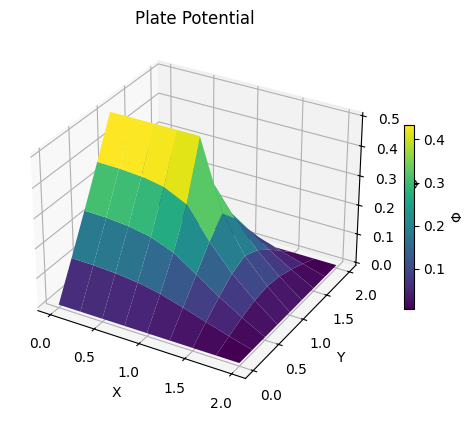
\includegraphics[width=0.49\linewidth]{images/surfaceplot1.png}
    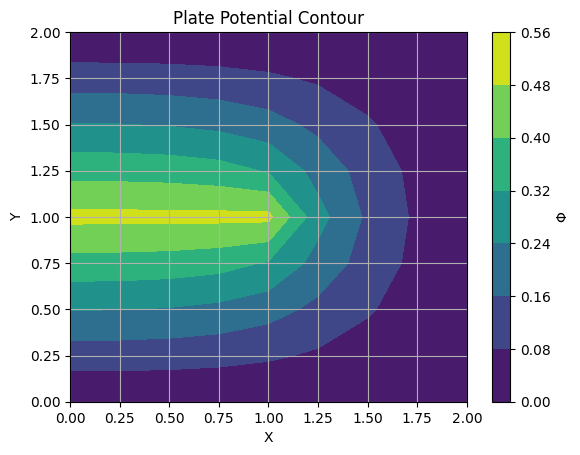
\includegraphics[width=0.49\linewidth]{images/contourplot1.png}
    \caption{Surface and contour plots for the approximate solution.}
\end{figure}

\begin{figure}
    \centering
    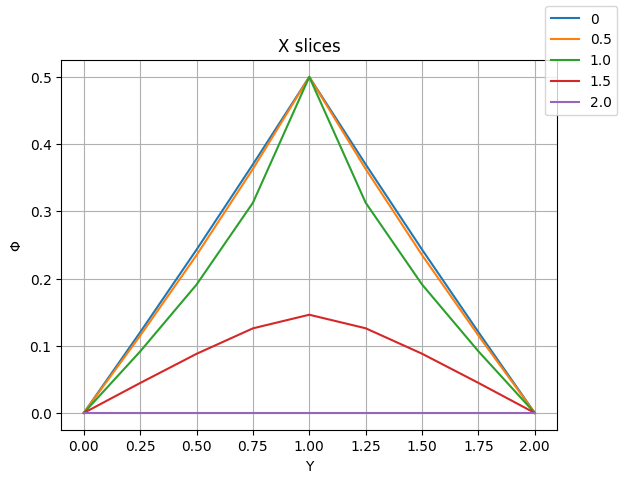
\includegraphics[width=0.49\linewidth]{images/xslice1.png}
    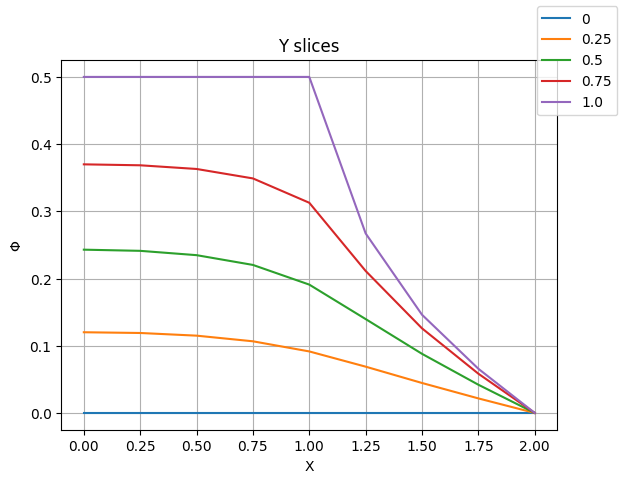
\includegraphics[width=0.49\linewidth]{images/yslice1.png}
    \caption{\(X\) and \(Y\) slices for the approximate solution.}
\end{figure}

\section{Computing the Electric Field}

The \(Y\)-component of the electric field in dimensionless units is \(\mathcal{E}_Y = -\pder[\Phi]{Y}\), which can be estimated as a finite difference by
\[ \mathcal{E}_Y(X, Y) \approx \pm\frac{1}{h} [\Phi(X, Y\mp h) - \Phi(X,Y)]. \]
Note that \(\mathcal{E}_Y\) may be have a jump discontinuity at \(Y = 1\), in which the left and right derivatives are not equal, but may be estimated by appropriate choice of the \(\pm\) signs.

Let us now take \(L = 2\), \(h = 1/4\) and \((D_X, D_Y) = (4, 4)\) and plot the numerical approximations of the potential \(\Phi(0, Y)\) and \(\Phi(2, Y)\), as well as the electric field \(\mathcal{E}_Y(X, 0)\) and \(\mathcal{E}_Y(X, Y \to 1^{\pm})\).

\begin{minted}[autogobble, linenos]{python}
    def compute_electric_field_on_plate(Phi, X, Y, h, Y_value):
        y_idx = np.argmin(np.abs(Y - Y_value))
        x_indices = np.arange(0, len(X))
        Ey_plus = -(Phi[y_idx + 1, x_indices] - Phi[y_idx, x_indices])
        Ey_minus = -(Phi[y_idx, x_indices] - Phi[y_idx - 1, x_indices])
        return X, Ey_plus / h, Ey_minus / h
\end{minted}

\begin{figure}
    \centering
    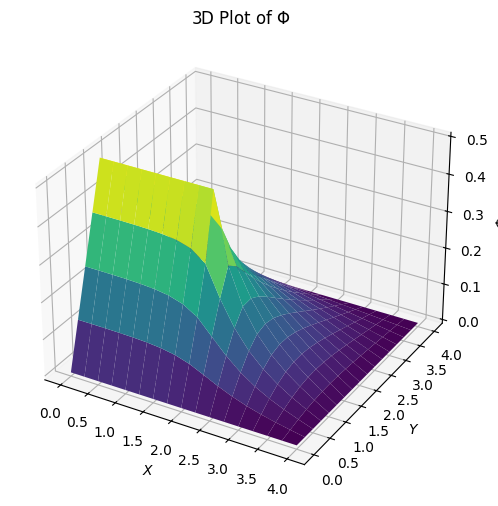
\includegraphics[width=0.49\linewidth]{images/surfaceplot2.png}
    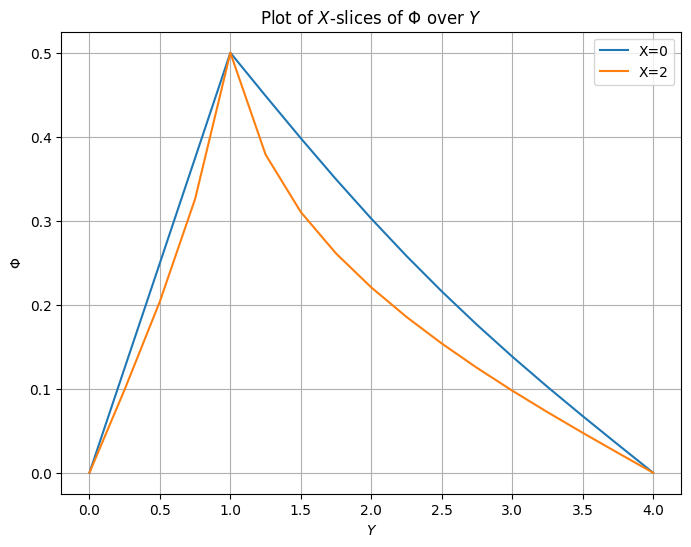
\includegraphics[width=0.49\linewidth]{images/slice2.png}
    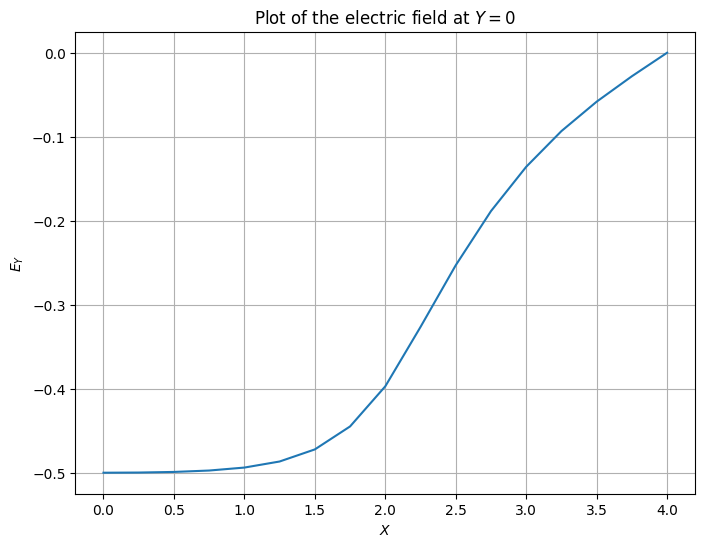
\includegraphics[width=0.49\linewidth]{images/electric2.png}
    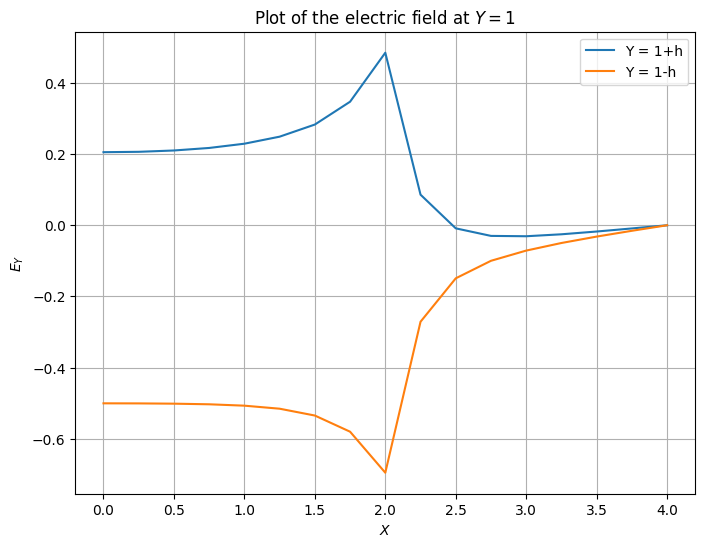
\includegraphics[width=0.49\linewidth]{images/plate2.png}
    \caption{Plots of the electric field.}
\end{figure}

Again, the accuracy is ensured using the residual, where the algorithm terminates after the residual drops below a preset value. The plot for the electric field at \(Y=0\) corresponds to decay as we move away from the plate. The two plots for the electric field at \(Y=1\) represent the charge signs at opposite faces of the plates which is shown by the discontinuity of left and right derivatives. There is a strong edge effect at \(X=2\) and a weak off the plate region as \(X \to 4\).

\begin{figure}
    \centering
    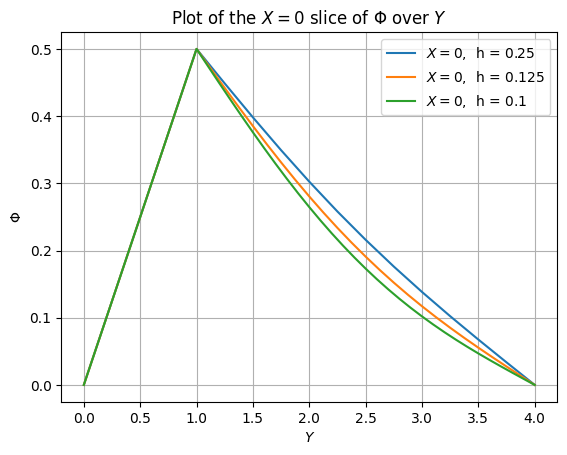
\includegraphics[width=0.49\linewidth]{images/slice0h3.png}
    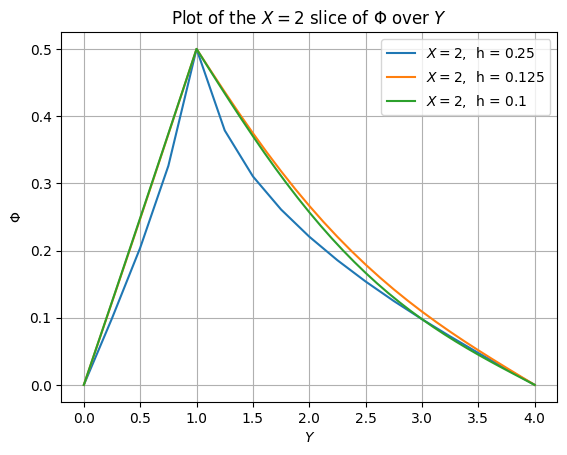
\includegraphics[width=0.49\linewidth]{images/slice2h3.png}
    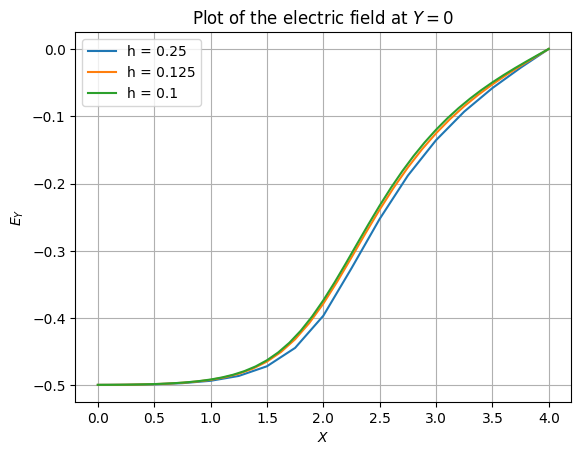
\includegraphics[width=0.49\linewidth]{images/efield0h3.png}
    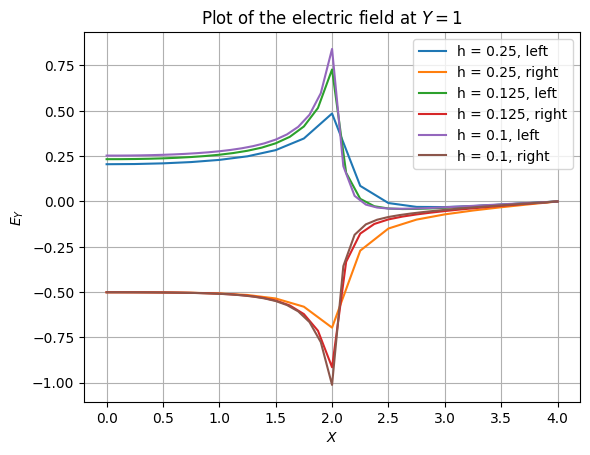
\includegraphics[width=0.49\linewidth]{images/efield1h3.png}
    \caption{Comparison of the slice plots when we decrease \(h\).}
\end{figure}

Varying \(h\) instead, we see that as \(h\) decreases, both \(X\) slices exhibit the following behaviour: the plot starts at \(0\) at the boundary condition at \(Y = 0\), increases to \(1/2\) at \(Y=1\) on the plate finally decreases back to \(0\) at \(Y=4\). Both the rise and decay portions seem to converge as we take \(h = 0\). We see similar convergence for the plots of the electric field. For \(Y = 0\), near the plate, field is relatively strong and away from the plate, the field is weak. This is demonstrated by the 'logistic' behaviour of the curve. For \(Y = 1\). we seem to see some blow-up at the plate \(X=2\) where the field lines concentrate at the plate edges. The two distinct curves correspond to the opposing sides of the plate when \(X < 2\) and since there is no physical plate when \(X > 2\), we see the two curves converging to one curve.

By looping the SOR algorithm for over-relaxation values \(\omega \in [1,2)\), we can analyse the number of iterations required for convergence.

\begin{figure}
    \centering
    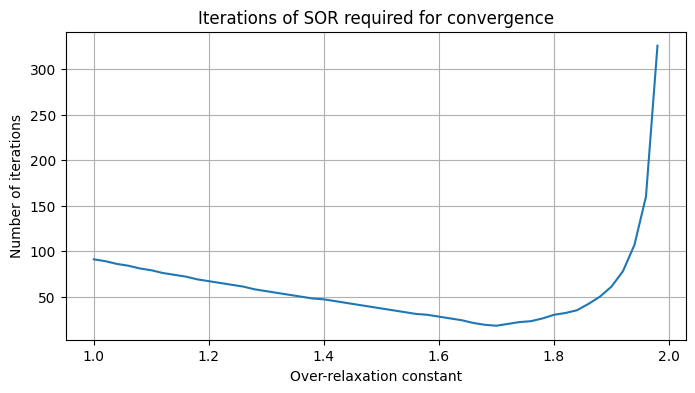
\includegraphics[width=1.0\linewidth]{images/relax.png}
    \caption{The number of iterations decreases until an optimal value, at which point it increases rapidly.}
\end{figure}

We see from the plot that the iterations starts relatively high at \(\omega = 1\) and then decreases to some optimal value. From there, the number of iterations increases rapidly as \(\omega \to 2\). It turns out that the optimal value for \(\omega\) our parameters on a square domain is 
\[ \omega_{\mathrm{opt}} = \frac{2}{1 + \sin(\pi h/D_X)} \approx 1.67, \]
which agrees with the minimum point on our plot. The actual optimal value may differ due to the geometry of the plates and imposition of mixed boundary conditions. Thus, empirical search is key to choosing a good over-relaxation constant.

\section{Computing the Charge}

In dimensionless units, the charge is given by
\[ Q = -\int_{\partial \Omega} (\nabla\Phi \cdot \mathbf{n})\,dS, \]
where \(\Omega\) is a domain containing exactly one of the plates. By the divergence theorem
\[ Q = -\int_{\Omega} \nabla^2 \Phi \,dV = -\int_{\Omega} \nabla^2 \Phi \,dX\,dY. \]
Inside the domain, but not on the plate, \(\nabla^2 \Phi = 0\) by the Laplace equation, so the charge only resides on the surface of the plates.

Let us consider \(\Omega\) to be a discrete grid of cells that enclose the plate at \(Y = Y_p\). Define the grid indices for \(M_L \leq m \leq M_R\) and \(N_B \leq n \leq M_T\). The integral is a sum of four integrals over the four sides of the rectangular boundary and the length of each segment \(dS\) on this discrete boundary is \(dX = dY = h\).

At the bottom boundary \(Y = N_B\). We have
\[ \nabla \Phi\cdot\mathbf{n} = \left(\pder[\Phi]{X}, \pder[\Phi]{Y}\right) \cdot (0, -1) = -\pder[\Phi]{Y}. \]
The integral over this bottom segment is
\[ \int_{X_{M_L}}^{X_{M_R}} \left.-\pder[\Phi]{Y}\right|_{Y = Y_B} \,dX. \]
Approximating the derivative
\[ \pder[\Phi]{Y} \approx \frac{\Phi_{i, N_B} - \Phi_{i, N_B - 1}}{h}, \]
we see the contribution from the bottom boundary is
\[ -\sum_{i=M_L}^{M_R} \frac{\Phi_{i, N_B} - \Phi_{i, N_B - 1}}{h}. \]
By computing the contributions from the other three boundaries, and summing them together, we obtain the approximation of the charge
\begin{eqnarray*} 
    Q & \approx & 
    \sum_{i=M_L}^{M_R}[\Phi_{i, N_B} - \Phi_{i, N_B-1} + \Phi_{i, N_T} - \Phi_{i, N_T+1}] \\
    & & + \sum_{j=N_B}^{N_T}[\Phi_{M_L, j} - \Phi_{M_L-1, j} + \Phi_{M_R, j} - \Phi_{M_R+1, j}].
\end{eqnarray*}
We can take \(M_L\) and \(M_R\) to be the left-most and right-most edges for the plate, \(X=0\) and \(X=L\). We then take \(N_B\) and \(N_T\) to be the indices one away from the plate \(Y=1\). 

\begin{minted}[autogobble, linenos]{python}
    def compute_charge(Phi, X, Y, h, L):
        y_plate_idx = np.argmin(np.abs(Y - 1.0))
        x_plate_idx = np.argmin(np.abs(X - L))
        N_B = y_plate_idx - 1
        N_T = y_plate_idx + 1
        M_L = 0
        M_R = x_plate_idx
    
        Q_term_1 = 0.0
        for i in range(M_L, M_R + 1):
            bottom = Phi[N_B, i] - Phi[N_B - 1, i]
            top = Phi[N_T, i] - Phi[N_T + 1, i]
            Q_term_1 += bottom + top
    
        Q_term_2 = 0.0
        for j in range(N_B, N_T + 1):
            # Symmetry Phi[-1, j] = Phi[1, j]
            left = Phi[j, M_L] - Phi[j, M_L + 1]
            right = Phi[j, M_R] - Phi[j, M_R + 1]
            Q_term_2 += left + right
        return Q_term_1 + Q_term_2
\end{minted}

Running this program, we obtain the approximations for the charge when we vary \(h\):
\begin{verbatim}[Output]
    h = [ 1/24   1/16   1/12   1/8    1/6    1/4   ]
    Q = [ 1.8586 1.8699 1.882  1.9069 1.9321 1.983 ]
\end{verbatim}
which seems to indicate monotone convergence of \(Q\) as \(h \to 0\). We tighten the tolerance to \(10^{-6}\) for the SOR method for lower values of \(h\), as the cumulative iteration error from summing many terms of \(\Phi\) may be large. Also, we use \(\omega = 1.5\) to reduce the number of iterations, improving performance.

Instead, by varying \(D_X\) and \(D_Y\) such that \(D_X = D_Y\), we can examine the behaviour of the boundary condition \(\Phi \to 0\) as \(|X|, |Y| \to \infty\).

\begin{figure}
    \centering
    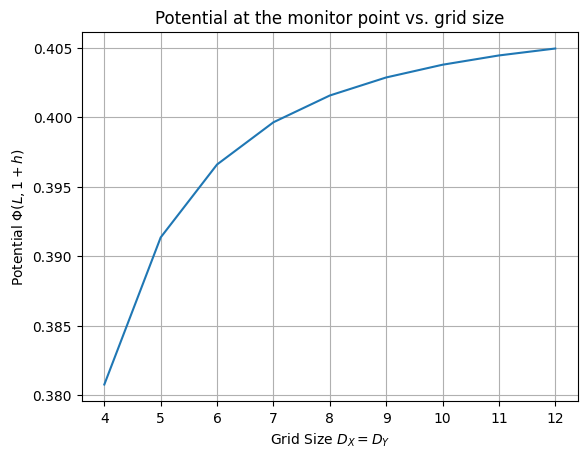
\includegraphics[width=0.49\linewidth]{images/monitor4.png}
    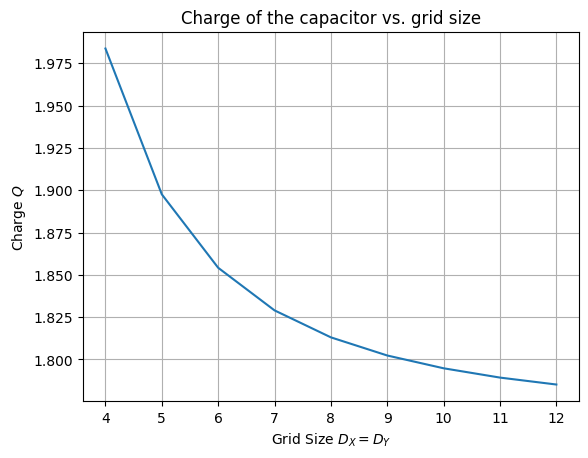
\includegraphics[width=0.49\linewidth]{images/charge4.png}
    \caption{Convergence of the charge and potential near the plate as \(D_X,D_Y \to \infty\).}
\end{figure}

At the monitor potential \(\Phi(L, 1+h)\) we see that as we increase the size of the quadrant, the potential is monotonically increasing and seems to converge. Likewise, the charge monotonically decreases and also seems to converge. When the domain is small, the artificial boundary is close to the plates which confines the electric field and pulls the potential down more aggressively. The influence of the boundary reduces as it moves away from the monitor potential. The flattening of the curve reflects the fact that the potential becomes less sensitive to a far away boundary. 

Analogously, when the domain is small, the close proximity of the boundary increases the capacitance of the system by bringing grounded plates closer to the charged plates. This charge decreases as the boundary moves away from the plates and also becomes less sensitive to a far away boundary.

\section{Equipotentials and Field lines for Semi-Infinite Plates}

To understand the behaviour of \(\Phi\) near the ends of the plates, we consider semi-infinite plates at \(Y =\pm 1\) with \(X \in (-\infty, L)\). The theory of conformal mappings provide analytic solutions for the equipotentials (lines of constant potential).

Define a function \(\Psi: \mathbf{R}^2 \to \mathbf{R}\) such that the lines of constant \(\Psi\) are everywhere orthogonal to the equipotentials. Now define \(W = -\Phi + i\Psi\) so that
\[ (X-L) + iY = \frac{1+e^{-2\pi iW}}{\pi} - 2iW. \] 
Equipotential lines can be computed parametrically by fixing \(\Phi \in  [-\frac{1}{2}, \frac{1}{2}]\), then varying \(\Phi\) and finally taking real and imaginary parts. Lines of constant \(\Psi\), known as field lines, are similarly computed by fixing \(\Psi\) and varying \(\Phi\). The value of \(L\) only shifts the field lines in the \(X\) direction.

The electric field \((\mathcal{E}_X, \mathcal{E}_Y) = (-\pder[\Phi]{X}, -\pder[\Phi]{Y})\) can be obtained from \(\Phi\) and \(\Psi\) via the following formula
\[ -\pder[\Phi]{X} + i\pder[\Phi]{Y} = \frac{i}{2(e^{-2\pi iW} + 1)}. \]

First, let us set \(L = 0\) so that the formula simplifies to
\[ X + iY = \frac{1+e^{-2\pi iW}}{\pi} - 2iW. \]
Substituting \(W = -\Phi + i\Psi\),
\begin{eqnarray*}
    X + iY & = & \frac{1+e^{-2\pi i(-\Phi + i\Psi)}}{\pi} - 2i(-\Phi + i\Psi) \\
           & = & \frac{1}{\pi}[1+e^{2\pi\Psi}(\cos(2\pi\Phi) + i\sin(2\pi\Phi))] + 2i\Phi + 2\Psi. 
\end{eqnarray*}
By separating the real and imaginary parts, we obtain
\[ X(\Phi, \Psi) = \frac{1}{\pi}[1 + e^{2\pi\Psi}\cos(2\pi\Phi)] + 2\Psi, \quad Y(\Phi, \Psi) = \frac{1}{\pi}[e^{2\pi\Psi}\sin(2\pi\Phi)] + 2\Phi. \]
Note that these satisfy the boundary conditions \(Y(\pm1/2, \Psi) = \pm1\) and we have 
\[ X(\pm 1/2, \Psi) = \frac{1}{\pi}[1-e^{2\pi \Psi}] + 2\Psi. \]
With the understanding that \(\Psi \in (0, \infty)\) is the upper surface and \(\Psi \in (-\infty, 0)\) is the lower surface, as \(\Psi \to -\infty\), we have \(X(\pm 1/2, \Psi) \to -\infty\), whilst as \(\Psi \to 0\), we have \(X(\pm 1/2, \Psi) \to 0\). This confirms that the edge of the semi-infinite plates is at \(X = 0\) and \(Y = \pm 1\).

We use the following function to plot some equipotential and field lines near the two plates.

\begin{minted}[autogobble, linenos]{python}
    def compute_equipotential_and_field_lines(Phi, Psi):
        exp_term = np.exp(2 * np.pi * Psi)
        cos_term = np.cos(2 * np.pi * Phi)
        sin_term = np.sin(2 * np.pi * Phi)
        X = (1 / np.pi) * (1 + exp_term * cos_term) + 2 * Psi
        Y = (1 / np.pi) * (exp_term * sin_term) + 2 * Phi
        return X, Y
\end{minted}

\begin{figure}
    \centering
    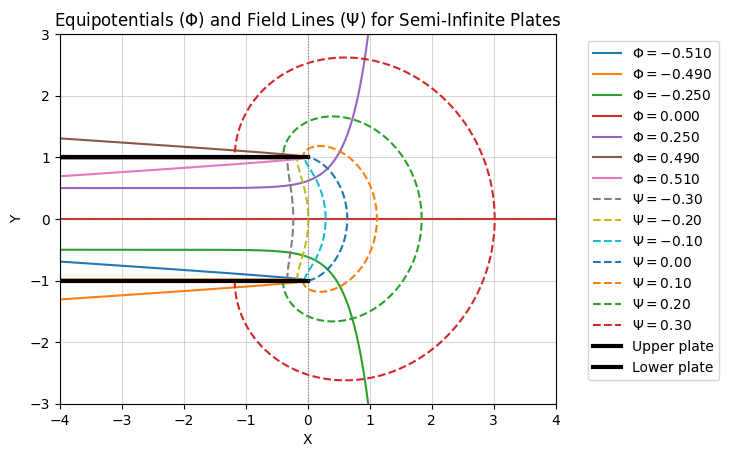
\includegraphics[width=1.0\linewidth]{images/equipfield.png}
    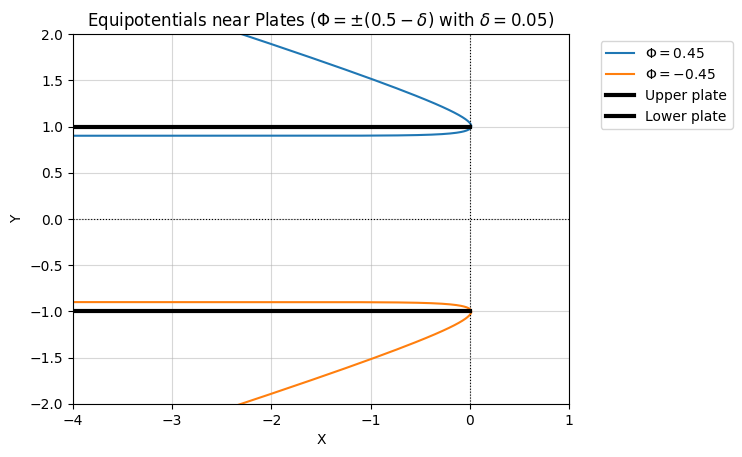
\includegraphics[width=1.0\linewidth]{images/equipnear.png}
    \caption{Equipotential and field lines are orthogonal near the semi-infinite plates.}
\end{figure}
Equipotentials broadly follow the plates for \(X < 0\), and then diverge away after the plate end. The orthogonal field lines emanate from the plate boundary and fringe outwards into the positive half-plane.

Evaluating the electric field at the upper surface of the top plate \(\Phi = 1/2\) from the formula
\[ \mathcal{E}_X - i\mathcal{E}_Y = -\pder[\Phi]{X} + i\pder[\Phi]{Y} = \frac{i}{2(e^{-2\pi iW} + 1)} \]
yield
\[ \frac{i}{2(e^{-2\pi i(-1/2 + i\Psi)} + 1)} = \frac{i}{2(e^{\pi i}e^{2\pi \Psi} + 1)} = \frac{i}{2(1 - e^{2\pi \Psi})}. \]
The real part is \(\mathcal{E}_X = 0\) and the imaginary part is \([2(e^{2\pi \Psi} - 1)]^{-1}\). This shows that the electric field is entirely in the \(Y\) direction with magnitude given by
\[ |\mathcal{E}| = \left|\frac{1}{2(e^{2\pi \Psi} - 1)}\right|, \]
and since we are on the upper surface, \(e^{2\pi \Psi}  >  1\).

As \(\Psi \to 0^+\), we are approaching the edge of the plate \(X = L^-\). We have the second order approximation \(e^{2\pi \Psi} \approx 1 + 2\pi\Psi + \frac{(2\pi\Psi)^2}{2}\), so \(\mathcal{E}_Y(X, 1^+) \approx \frac{1}{4\pi\Psi}\). Now
\begin{eqnarray*}
    X - L & = & \frac{1}{\pi}(1 - e^{-2\pi\Psi}) + 2\Psi \\
          & \approx & \frac{1}{\pi}\left(1 - \left(1 + 2\pi\Psi + \frac{(2\pi\Psi)^2}{2}\right)\right) + 2\Psi \\
          & \approx & \frac{1}{\pi}\left(-2\pi\Psi - 2\pi^2\Psi^2\right) + 2\Psi \\
          & \approx & -2\pi\Psi^2.
\end{eqnarray*}
Since \(\Psi > 0\), this means that \(\Psi \approx \sqrt{\frac{L-X}{2\pi}}\), which implies
\[ \mathcal{E}_Y(X, 1^+) \approx \frac{1}{4\pi\sqrt{\frac{L-X}{2\pi}}} = \frac{1}{\sqrt{8\pi(L-X)}}. \]

As \(\Psi \to \infty\), we are moving far to the left along along the plate \(X \to -\infty\) and \(e^{2\pi\Psi} - 1 \approx e^{2\pi\Psi}\) is very large, so \(\mathcal{E}_Y(X, 1^+) \approx [2e^{2\pi\Psi}]^{-1}\) and \(X - L \approx -\frac{1}{\pi}e^{2\pi\Psi}\). Therefore,
\[ \mathcal{E}_Y(X, 1^+) \approx \frac{1}{2\pi(L-X)}. \]

On the lower surface (opposite side) of the top plate \(\Psi < 0\), as \(\Psi \to 0^-\) which means \(X \to L^-\), the sign of the electric field flips as now the denominator satisfies \(e^{2\pi\Psi} - 1 < 0\). This means that close to the edge, the electric field on the upper and lower surfaces of the plate are equal in magnitude but have opposite sign. In contrast, as \(\Psi \to -\infty\) which means \(X \to -\infty\), the exponential term now is very small \(1 - e^{2\pi \Psi} \to 1\), so the magnitude of the electric field approaches \(\frac{1}{2}\), hence \(\mathcal{E}_Y(X, 1^-) \approx -\frac{1}{2}\). This means that far from the edge, the electric field on the lower surface is uniform and points in the negative direction.

To summarise, for the top plate \(\Phi = \frac{1}{2}\):
\begin{enumerate}
    \item The electric field in the \(X\) direction is zero, \(\mathcal{E}_X = 0\).
    \item The \(Y\) component, hence the entire electric field is given by
    \[ \mathcal{E} = \frac{1}{2(e^{2\pi \Psi} - 1)}. \]
    \item On the upper surface of the top plate, \(\mathcal{E}_Y(X, 1^+)\), the surface corresponds to \(\Phi > 0\). Near the edge \(X \to L^-\), corresponding to \(\Phi \to 0^+\), 
    \[ \mathcal{E}_Y(X, 1^+) \approx \frac{1}{\sqrt{8\pi(L-X)}}, \]
    where the field becomes infinitely strong and points upwards. Away from the edge \(X \to -\infty\), corresponding to \(\Phi \to \infty\),
    \[ \mathcal{E}_Y(X, 1^+) \approx \frac{1}{2\pi(L-X)}, \]
    where the field points upwards and decays.
    \item On the lower surface of the top plate, \(\mathcal{E}_Y(X, 1^+)\), the surface corresponds to \(\Phi < 0\). Near the edge \(X \to L^-\), corresponding to \(\Phi \to 0^-\), 
    \[ \mathcal{E}_Y(X, 1^+) \approx -\frac{1}{\sqrt{8\pi(L-X)}}, \]
    where the field becomes infinitely strong and points downwards. Away from the edge \(X \to -\infty\), corresponding to \(\Phi \to -\infty\),
    \[ \mathcal{E}_Y(X, 1^+) \approx -\frac{1}{2}, \]
    where the field points downwards and has uniform strength.
\end{enumerate}

\section{Comparison of Semi-Infinite Plates with Finite Plates}

Let us take large (relative to the plate separation) values of \(L = 2,3,4\) and then take \(D_X = D_Y = L + 4\) to minimise the effect of artificial boundaries. Also, set \(\omega = \frac{5}{3}\) and \(h = \frac{1}{4}\) to improve performance. We run the SOR method and compare the electric field on the upper and lower surface of the top plate to the analytic formula \(\mathcal{E}_Y(X, 1^{\pm})\).

\begin{figure}
    \centering
    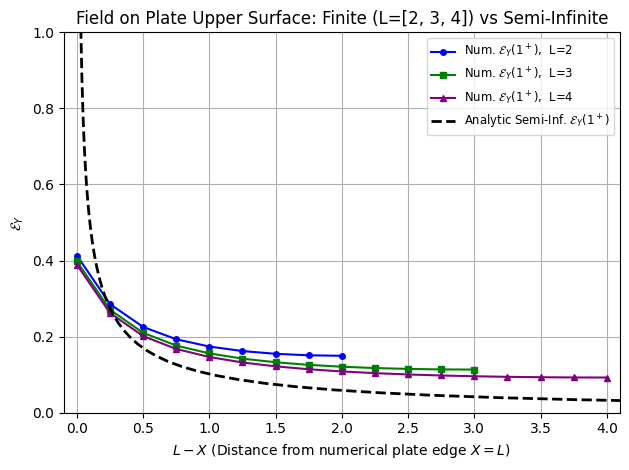
\includegraphics[width=0.49\linewidth]{images/semiinf1.png}
    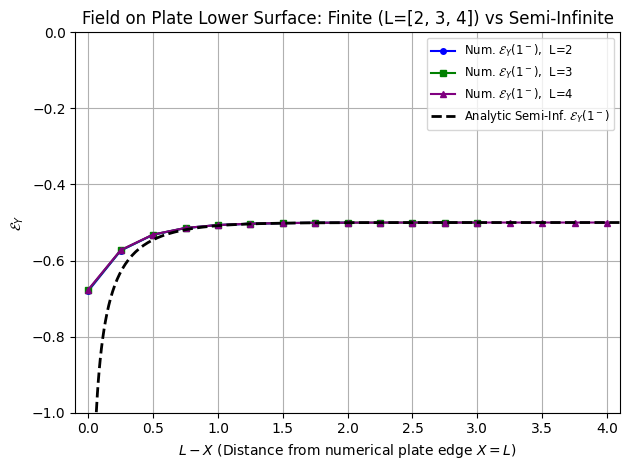
\includegraphics[width=0.49\linewidth]{images/semiinf2.png}
    \caption{Convergence of the finite case to the semi-infinite case.}
\end{figure}

For a given edge at \(X = L\), the numerical solution for the finite plate matches the semi-infinite analytical solution closely, and as \(L \to  \infty\), we have convergence since the influence from the other edge at \(X = -L\) becomes negligible. Conversely, the match will be poor at the other edge or at \(X = 0\). As \(L\) increases, the region of good agreement near each edge should extend further inwards from that edge.

\begin{minted}[autogobble, linenos]{python}
    def get_analytical_Ey_semi_infinite(Psi_values, L):
        X = L + (1 / np.pi) * (1 - np.exp(2 * np.pi * Psi_values)) 
        extra_term = 2 * Psi_values
        X_abs = L + X + extra_term
        E_Y = 1 / (2 * (np.exp(2 * np.pi * Psi_values) - 1))
        return X_abs, E_Y, X + extra_term
\end{minted}

More precisely, on the lower surface we see the analytic solution has the \((L-X)^{-1/2}\) singularity as \(L-X \to 0\), approaching the edge \(\mathcal{E}_Y \to -\infty\). On the other hand, as \(L-X \to \infty\), we see the uniform field \(\mathcal{E}_Y \to -\frac{1}{2}\). Near the edge, the finite numerical solutions closely follow the analytic solution, deviate as we move away from the edge before settling off again at \(\mathcal{E}_Y \approx -\frac{1}{2}\). This deviation is not visibly present in our plots, owing to the large values of \(L\).

For the upper surface, we have the flipped singularity for the analytic solution close to the plate, but as we move away from the plat \(L-X \to \infty\), as have \((L-X)^{-1}\) decay, meaning the field always decays to zero. Again, near the edge, the numerical solutions for the finite plates closely follow the analytic curve and deviate as we move away from the plate. The influence of the other edge causes the numerical curve to flatten out, rather than decay to zero.

\end{document}
